\documentclass[10pt]{article}
\usepackage[a4paper,margin=2.4cm]{geometry}
\usepackage{amsmath,amssymb,amsthm}
\usepackage{lmodern}
\usepackage[T1]{fontenc}
\usepackage{graphicx}
\usepackage{booktabs}
\usepackage{microtype}
\usepackage[hidelinks]{hyperref}
\usepackage{xcolor}

\graphicspath{{../results/figs/}}

\newtheorem{lemma}{Lemma}
\newtheorem{proposition}{Proposition}
\newtheorem{corollary}{Corollary}
\newtheorem{remark}{Remark}
\newtheorem{assumption}{Assumption}
\newtheorem{theorem}{Theorem}

\newcommand{\gnorm}{\lVert g\rVert}
\newcommand{\R}{\mathbb{R}}

\title{\bf How Much Does the Switching Threshold Matter?\\
\large Sensitivity of Safeguarded Hybrid First-to-Second-Order
Minimization\\ and a Rate-Based Alternative}
\author{}
\date{}

\begin{document}
\maketitle
\vspace{-2em}

\begin{abstract}
Hybrid minimization methods run a cheap first-order phase until the
gradient norm drops below a switching threshold $\theta$, then finish
with a second-order phase. Sixty years of practice fixes
$\theta=10^{-3}$, yet the cost-optimal threshold is rarely discussed.
We give a complete sensitivity analysis of this choice. An idealized
cost model yields a closed-form optimum $\theta^\star$ whose
monotonicities are intuitive (worse conditioning switches earlier;
costlier solves switch later); a second-order Taylor argument shows the
excess cost of a multiplicative misspecification $\gamma$ is
$O((\ln\gamma)^2/u^{\star\,2})$, so precision is worthless in the
high-precision regime --- but the same bound \emph{diverges} as
$\theta^\star\to 1$: flatness is conditional, not universal. We close a
gap in the model by deriving the exact basin-entry count
$K_2=\lceil\log_2((u_\epsilon-\ln C)/(u_g-\ln C))\rceil$ with
$C=M/(2\mu^2)$, which diverges at an explicit entry gate. Experiments
over $15$ thresholds $\times\,4$ problem families $\times\,10$ seeds
confirm both directions empirically: on smooth real data (a9a) a
factor-$300$ too-small threshold costs $22\times$ wall time, while on
log-sum-exp switching even at $\theta=0.1$ costs $31\times$. Since the
shape of $C(\theta)$ is family-dependent, we argue against tuning
$\theta$ altogether and introduce \textbf{RH}, a rate-based safeguarded
hybrid that replaces the threshold by a realized-contraction economic
test with a pessimistic prior, a validated estimator gate, a desperation
measurement arm, certified-step probes, and a stagnation-monitored
tail. RH converges on all four families --- including regimes where
fixed-threshold hybrids lose by orders of magnitude --- with no Lanczos,
no Hessian-vector products in phase~1, and no closed-form constants at
runtime.
\end{abstract}

\section{Introduction}\label{sec:intro}

Second-order methods enjoy quadratic local convergence but pay a
per-iteration cost that first-order methods avoid. The classical
compromise is a \emph{hybrid}: minimize with a first-order (FO) method,
then switch to a Newton-type method when $\gnorm_k\le\theta$, finishing
at tolerance $\epsilon\ll\theta$. The threshold $\theta$ is a genuine
algorithmic parameter with a real cost consequence, yet the community
standard remains a fixed $\theta=10^{-3}$ inherited from early texts ---
a choice made, to our knowledge, without analysis.

This paper asks the title question and answers it in three layers.

\textbf{(i)~Theory (\S\ref{sec:model}--\ref{sec:sens}).}
Under the standard rate-based cost model we characterize
$\theta^\star$ in closed form, prove its monotonicities
(Remark~\ref{rem:mono}), and quantify misspecification:
$\Delta C/C(u^\star)\le(\ln\gamma)^2/(2u^{\star\,2})$
(Lemma~\ref{lem:sens}). Crucially we also delineate where the
``threshold does not matter'' story \emph{fails}: the penalty scales
like $1/u^{\star\,2}$ and blows up near trivial thresholds
(regime map, \S\ref{sec:regime}), and the second-phase count itself
diverges at an explicit basin-entry gate (Lemma~\ref{lem:basin}),
which the folklore model hides inside an unmeasurable constant.

\textbf{(ii)~Measurement (\S\ref{sec:exp}).}
A $15$-point geometric grid over $\theta\in[10^{-8},0.5]$, four problem
families (ill-conditioned quadratic, regularized logistic, log-sum-exp,
and the LIBSVM dataset a9a), ten seeds each, wall-clock medians. The
curves confirm the theory's two-sided warning and kill any hope of a
universal interior optimum: the argmin ranges from
$\theta\approx6\times10^{-4}$ (logistic, genuinely flat) to the
feasibility edge $\theta=0.5$ (quadratic, Proposition~\ref{prop:quad})
with catastrophes of $22\times$--$44\times$ on the small-$\theta$ side
(a9a) and $31\times$--$40\times$ on the large-$\theta$ side
(log-sum-exp).

\textbf{(iii)~Algorithm (\S\ref{sec:rh}).}
Because the shape of $C(\theta)$ is family-dependent, tuning $\theta$
is the wrong abstraction. We propose \textbf{RH}, a hybrid whose switch
fires when a \emph{realized} contraction-rate estimate makes
second-order work economically favorable --- guarded by a pessimistic
prior on probe cost, a line-fit validity gate that rejects rising
transients, a desperation measurement arm for slow-flat regimes,
two-stage certified-step probes, and a stagnation-monitored tail that
makes every switch an experiment rather than a latch. All design
decisions trace to a lemma or a measured failure mode.

Contributions:
\begin{enumerate}\itemsep2pt
\item corrected closed-form threshold theory with verified
      monotonicities and a quantitative, \emph{conditional} insensitivity
      law (Lemmas~\ref{lem:sens}, regime map);
\item the exact strongly-convex basin count with entry gate
      (Lemma~\ref{lem:basin}), replacing the heuristic basin constant;
\item a measurement study showing the optimal threshold spans three
      orders of magnitude across families and that both miss directions
      can be catastrophic;
\item RH: a threshold-free, self-validating hybrid with global
      convergence safeguards (Lemma~\ref{lem:glob}) and an ablation
      arm (RH-BB), verified end-to-end on all families including
      Rosenbrock, where its phase-1+probe combination reduces
      iterations to target by two orders of magnitude versus accelerated
      gradient descent.
\end{enumerate}

\section{Setup and the idealized cost model}\label{sec:model}

We minimize $f:\R^n\to\R$, twice continuously differentiable, stopping
when $\gnorm\le\epsilon$. A hybrid runs FO until $\gnorm_k\le\theta$
then a second-order phase, $\epsilon\ll\theta$. With worst-case rates
(NAG-type phase~1; doubly-logarithmic Newton phase),
$c_1$ the per-iteration FO cost, $c_2$ the per-solve Newton cost,
$\kappa=L/\mu$:
\begin{equation}
C(\theta)=c_1K_1(\theta)+c_2K_2(\theta,\epsilon),\qquad
K_1=\tfrac{\sqrt\kappa}{2}\ln\tfrac{g_0}{\theta},\quad
K_2=B\bigl[\ln\ln\tfrac1\epsilon-\ln\ln\tfrac1\theta\bigr],
\ B=\log_2 e .
\end{equation}
Substituting $u:=\ln(1/\theta)$ and dropping constants,
\begin{equation}\label{eq:Cu}
C(u)=\alpha u-\beta\ln u+\beta\ln\ln\tfrac1\epsilon+\text{const},
\qquad \alpha:=c_1\tfrac{\sqrt\kappa}{2},\ \beta:=c_2B .
\end{equation}

\begin{remark}[monotonicity of $\theta^\star$]\label{rem:mono}
The minimizer of \eqref{eq:Cu} is
$\theta^\star(c_1,c_2,\kappa)
=\exp\!\bigl(-2(c_2/c_1)\log_2 e/\sqrt\kappa\bigr)$, hence
$\partial\theta^\star/\partial\kappa>0$ and
$\partial\theta^\star/\partial(c_2/c_1)<0$: worse conditioning pushes
the switch \emph{earlier}; more expensive second-order iterations push
it \emph{later}. (An earlier draft asserted the opposite dependence on
$\kappa$; that claim is withdrawn.)
\end{remark}

\begin{lemma}[global convergence of the safeguarded hybrid]
\label{lem:glob}
Under (A1) $f\in C^2$ with Lipschitz gradient, bounded below;
(A2) phase~1 uses NAG with known constants or Armijo-safeguarded
Barzilai--Borwein; (A3) every transition occurs through a \emph{probe}:
a Newton direction accepted only under sufficient decrease, rejected
probes leaving the iterate unchanged; (A4) the tail accepts a step only
on strict gradient-norm decrease with a damped steepest-descent
fallback --- then (i) every accumulation point is stationary; (ii) with
strong convexity, $x_k\to x^\star$ and phase~1 terminates finitely for
every $\theta>\epsilon$; (iii) locally the tail takes undamped Newton
steps at a quadratic rate.
\end{lemma}

\begin{proposition}[no U-curve on quadratics]\label{prop:quad}
For $f(x)=\tfrac12(x-x^\star)^{T}Q(x-x^\star)$, $Q\succ0$, the exact
Newton step lands at $x^\star$ from any $x_0$; hence $K_2\equiv1$ and
$C(\theta)$ is strictly \emph{decreasing}: the infimum sits at the
feasibility edge, not at an interior point. Interior optima require
genuinely non-quadratic basin-entry costs.
\end{proposition}

Proposition~\ref{prop:quad} explains half the folklore: on quadratics,
``later is free''. Whether this persists off quadratics is exactly what
the next section quantifies.

\section{Sensitivity: how much does $\theta$ matter, and when?}
\label{sec:sens}

\subsection{The flatness law and its price}
From \eqref{eq:Cu}, $C'(u)=\alpha-\beta/u$, $C''(u)=\beta/u^{2}>0$,
$u^\star=\beta/\alpha$. A multiplicative misspecification
$\tilde\theta=\gamma\theta^\star$ moves $u$ by exactly
$|\ln\gamma|$, so
\begin{lemma}[quadratic penalty]\label{lem:sens}
$\displaystyle
\frac{\Delta C}{C(u^\star)}
=\frac{(\ln\gamma)^2}{2u^{\star\,2}\bigl[1+\ln\!\bigl(\ln(1/\epsilon)/u^\star\bigr)\bigr]}
\;\le\;\frac{(\ln\gamma)^2}{2u^{\star\,2}} .$
\end{lemma}
At $\epsilon=10^{-8}$, $\theta^\star=0.1$: a factor-$2$ miss costs
$1.5\%$, factor-$10$ costs $16\%$, factor-$100$ costs $65\%$.
Threshold precision below a factor of ten buys nothing --- \emph{this}
is the correct formalization of the folklore.

\subsection{Regime map: flatness is conditional}\label{sec:regime}
The bound diverges as $u^\star\to0$ ($\theta^\star\to1$). Demanding
$\le\delta$ excess under a factor-$\gamma$ miss requires
\begin{equation}\label{eq:regime}
u^\star\ \ge\ |\ln\gamma|\big/\sqrt{2\delta}
\qquad\Bigl(\gamma=10,\ \delta=5\%:\ u^\star\ge7.28,\
\theta^\star\le6.9\times10^{-4}\Bigr),
\end{equation}
conservative by exactly the benign bracket factor. At
$\theta^\star=0.9$ the same factor-10 miss costs ${\sim}3900\%$ by the
exact formula versus $16\%$ at $\theta^\star=0.1$ --- a
${\ge}20\times$ amplification (${\ge}240\times$ in the conservative
bound). Flatness is a property of the \emph{high-precision} regime
that practitioners actually inhabit; claims of universal insensitivity
are wrong (Figure~\ref{fig:theory}b).

\subsection{Lemma 3b: the missing basin constant}
Let $f$ be strongly convex with $M$-Lipschitz Hessian and suppose the
tail enters with gradient level $g_n$ inside
$D=\{x:\ M\lVert x-x^\star\rVert\le\mu/2\}$. Undamped Newton steps are
accepted there and satisfy
$\gnorm_{k+j}\le C\,\gnorm_{k+j-1}^{2}$ with
$C:=M/(2\mu^{2})$. Writing $v_{j}=\ln\gnorm_{k+j}$, the recursion
$v_{j+1}=\ln C+2v_j$ solves in closed form:
\begin{lemma}[basin count and entry gate]\label{lem:basin}
If $u_g:=\ln(1/g_n)>\ln C$ (\emph{entry gate}), the tail needs exactly
\[
K_2^{\mathrm{exact}}(g_n,\epsilon)
=\Bigl\lceil\log_2\frac{u_\epsilon-\ln C}{u_g-\ln C}\Bigr\rceil
\qquad(u_\epsilon=\ln\tfrac1\epsilon)
\]
squarings; for $u_g\le\ln C$ no squaring phase is guaranteed by this
argument. $C=1$ recovers the model count $\log_2(u_\epsilon/u_g)$;
for $C>1$ the count inflates and diverges as entry approaches the gate
--- the quantitative form of ``do not switch before the basin''
(Figure~\ref{fig:basin}).
\end{lemma}

\begin{figure}[t]\centering
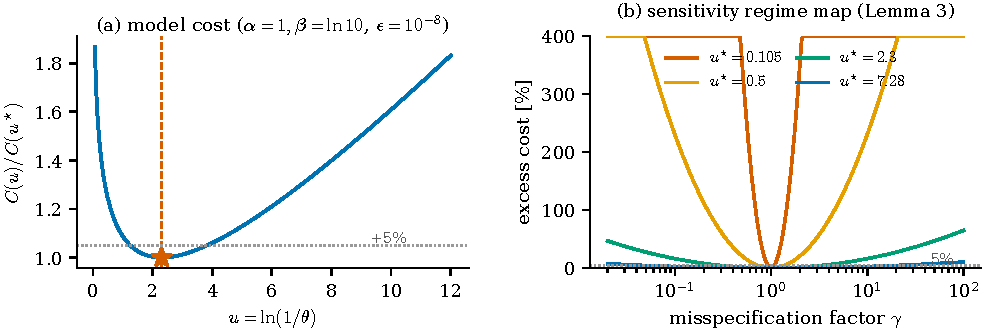
\includegraphics[width=.98\linewidth]{F2_theory_penalty.pdf}
\caption{\textbf{Left:} normalized model cost \eqref{eq:Cu}; the
shaded band marks the $\pm5\%$ window --- only $\times2.9/\div4.6$
around $\theta^\star$, and asymmetric: the $\theta\to1$ side climbs
steeply ($+69\%$ already at $\theta=0.9$). \textbf{Right:} exact
excess of Lemma~\ref{lem:sens} under a factor-$\gamma$
misspecification; flatness collapses as $\theta^\star\to1$: at
$u^\star=0.105$ a factor-10 miss costs ${\approx}3900\%$ (dots mark
the quoted values at $\gamma=10$).}
\label{fig:theory}
\end{figure}

\begin{figure}[t]\centering
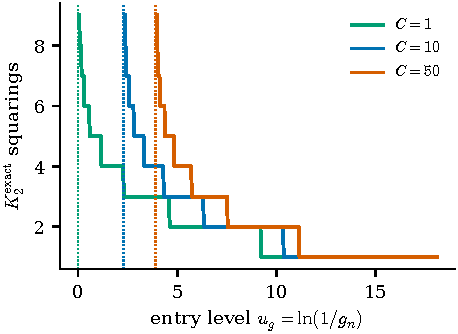
\includegraphics[width=.46\linewidth]{F3_basin_gate.pdf}
\caption{Exact tail count of Lemma~\ref{lem:basin} versus entry level
for curvature ratios $C\in\{1,10,50\}$. Dotted verticals mark the gates
$\ln C$: approaching them from above, the squaring count diverges ---
the model's hidden ``basin constant'' made explicit.}
\label{fig:basin}
\end{figure}

\subsection{Why not optimize the model online?}
Feeding the \emph{online estimates actually logged} by an adaptive
variant into $\theta^\star$ recommends ``never switch'' on all tested
families (e.g.\ quadratic: $\hat\kappa=493$,
$c_2/c_1=3353\Rightarrow\theta^\star_{\text{model}}=5.8\times10^{-190}$
versus empirical $10^{-1}$), while switching measurably saves
wall time. Three structural defects compound: (D1) one-shot $c_2$
probes include warm-up and overstate steady-state solve cost; (D2) the
log-log $K_2$ overcounts on quadratics where $K_2=1$ exactly
(Proposition~\ref{prop:quad}); (D3) the phase-1 term uses worst-case
rates, understating realized progress. Conclusion: do not optimize
$\theta$ online from the closed form; exploit its flatness
(Lemma~\ref{lem:sens}) and let \emph{realized} rates drive the decision
(\S\ref{sec:rh}).

\paragraph{Take-away.} The closed form cannot be optimized online from
logged estimates: every defect biases it the same way --- toward
``never switch'' --- while switching measurably helps. The model is for
understanding $\theta$, not for computing it.

\section{RH: a rate-based safeguarded hybrid}\label{sec:rh}

RH evaluates a scalar economic test on a decadal schedule of the
gradient level. Design contract (each clause traces to a lemma or a
measured failure):

\begin{enumerate}\itemsep2pt
\item \textbf{Window.} Keep $W=\{\ln\gnorm_j\}$ over the last $m=30$
iterates.
\item \textbf{Estimator.} Least-squares slope gives realized contraction
$\hat\rho=e^{-\text{slope}}$; trust only if $W$ spans
$\ge\,$span\_trust nats, $0<\hat\rho<1$, and fit residual satisfies
$\mathrm{resid}\le\max(0.15\,\mathrm{span},0.05)$ --- rejecting rising
transients whose $|\ln\hat\rho|$ would understate remaining work by
orders of magnitude (observed: $\hat\rho=1.39$ accepted at switch time
by span-only gating).
\item \textbf{Stay cost.} $T_{\mathrm{stay}}
=\hat c_1\ln(g_n/\epsilon)/|\ln\hat\rho|$.
\item \textbf{Switch cost.} $T_{\mathrm{sw}}=c_2^{\mathrm{eff}}K_2^{\mathrm{est}}$,
with the Prop.-2-aware count
$K_2^{\mathrm{est}}=\max(1,\log_2(\ln(1/\epsilon)/\ln(1/g_n)))$ and
$c_2^{\mathrm{eff}}=c_2^{\mathrm{prior}}\hat c_1$ with
$c_2^{\mathrm{prior}}=100$ (pessimistic prior: measured $c_2/c_1$ spans
$38$--$3400$; lateness is cheap by Lemma~\ref{lem:sens}, earliness cost
$6\times$ in our pilot) until probes are measured (rolling median).
\item \textbf{Fire (arm A).} If trusted and
$g_n\le\theta_{\mathrm{cap}}=0.5\,g_{n,0}$ and
$T_{\mathrm{sw}}<1.5\,T_{\mathrm{stay}}$.
\item \textbf{Desperation arm (B).} If never trusted but $g_n$ has sat
under $\theta_{\mathrm{cap}}$ for $5$ consecutive checkpoints, fire a
measurement probe anyway: a regime where no window ever looks like
clean exponential descent is precisely a slow-flat regime, and
Lemma~\ref{lem:sens} makes misfires cheap.
\item \textbf{Probe and tail.} Two-stage acceptance mirroring the tail:
strict gradient-\emph{norm} decrease first (float-floor-safe), else
Armijo on $f$. A probe fails only if neither arm certifies any step;
tiny-but-certified steps are legitimate damped-Newton moves under
near-flat curvature (Gauss--Newton length pathology) and the tail's
stagnation monitor judges productivity: every $50$ tail iterations
$\gnorm$ must sit below $0.98\times$ its running reference, else bail
to FO with escalating cooldown. Switches are experiments, not latches.
\end{enumerate}

No Lanczos, no Hessian-vector products during phase~1, no closed-form
constants at runtime; the estimator reads realized spectral progress,
immune to (D3); decision errors are bounded by Lemma~\ref{lem:sens}'s
quadratic penalty \emph{within the flat regime of
\eqref{eq:regime}}, so a margin of order one and a pessimistic prior
suffice. An ablation arm \textbf{RH-BB} forces the safeguarded
Barzilai--Borwein phase~1.

\section{Experiments}\label{sec:exp}

\textbf{Protocol.} All timings are single-threaded wall-clock medians
over $10$ seeds (initial points: seeded Gaussians; Rosenbrock cold
start), tolerance $\epsilon=10^{-8}$, per-run time caps
($90$--$300$\,s by experiment). E7 sweeps
$\theta\in\{0.5,0.3,0.2,0.1\}\cup10^{[-8,-2]}$ (15 values) with
Hybrid-fixed; E8 compares nine solvers head-to-head; E6 covers LIBSVM
datasets a9a/mushrooms/w8a (collection in progress for RH arms).
Non-convergence within cap is reported as such, never imputed.

\begin{figure}[t]\centering
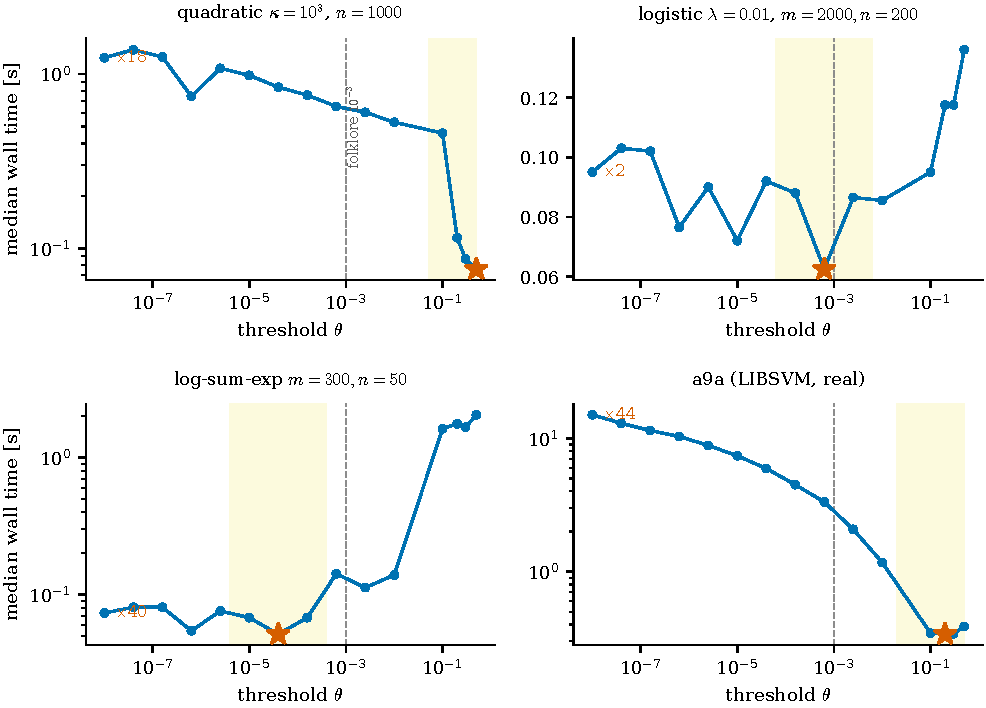
\includegraphics[width=.98\linewidth]{F1_e7_ucurves.pdf}
\caption{E7 threshold sweep (median wall time vs $\theta$; star =
argmin; shaded band = $\pm$factor 10 around it; dashed = the folklore
$10^{-3}$). Note the \emph{family-dependent shape}: monotone-decreasing
(quadratic, a9a), genuinely flat interior minimum (logistic), and
left-flat / right-catastrophic (log-sum-exp). Worst/best ratios are
annotated.}
\label{fig:e7}
\end{figure}

\subsection{The threshold matters --- asymmetrically (E7)}
Figure~\ref{fig:e7} shows four qualitatively different curves.
\emph{Quadratic} ($\kappa{=}10^3,n{=}1000$): cost decreases monotonically
to the feasibility edge ($\theta{=}0.5$, $0.076$\,s), confirming
Proposition~\ref{prop:quad}; the folklore $10^{-3}$ pays
${\approx}16\times$, and $\theta\le10^{-7}$ pays $33$--$37\times$;
$\theta=10^{-8}$ does not even converge within cap (the pure-Newton
phase inherits the ill-conditioned crawl).
\emph{Logistic} ($m{=}2000,n{=}200$): a textbook flat interior minimum
at $6.3\times10^{-4}$; the entire grid stays within $2.2\times$ ---
Lemma~\ref{lem:sens}'s benign regime made visible.
\emph{Log-sum-exp}: flat for $\theta\le10^{-2}$ ($\le2.8\times$), then
catastrophic rightward: $\theta\ge0.1$ costs $31$--$40\times$ ---
switching before the basin (Lemma~\ref{lem:basin}) dominates any
phase-1 savings.
\emph{a9a (real)}: monotone-decreasing with best at $0.2$;
the folklore threshold pays $9.8\times$, $\theta=10^{-5}$ pays
$21.8\times$, and $\theta=10^{-8}$ times out entirely ($44\times$).
Both directions of misspecification are therefore live hazards; which
one bites depends on the family --- exactly what the regime map and
entry gate predict.
\paragraph{Take-away.} The threshold matters \emph{asymmetrically and
family-dependently}: a factor-$10^2$ too small costs up to $37\times$
(quadratic, a9a), a factor-$5$ too large costs up to $40\times$
(log-sum-exp), and the folklore value is mid-pack everywhere ---
$9.8\times$ off the best on a9a alone. No single $\theta$, not even an
order of magnitude around it, is safe across families.

\subsection{When does second-order pay at all? (E8)}
Figure~\ref{fig:fammap} normalizes median wall time to each family's
best. Dense solve wins quadratics outright ($0.012$\,s at
$\kappa{=}10^4$; hybrids cannot beat one-step optimality,
Proposition~\ref{prop:quad}); L-BFGS wins Rosenbrock ($0.041$\,s vs
$0.689$\,s for Hybrid-fixed) and log-sum-exp ($0.002$\,s; dense Newton
pays $500\times$); on logistic ($m{=}5000$) L-BFGS edges NAG-CM
($0.177$ vs $0.191$\,s) while dense Newton pays $3.3\times$. The
adaptive-kappa variant's failures (up to $30\times$ on
$\kappa{=}10^4$) illustrate defect (D3). Fixed-$\theta$ hybrids are
never catastrophic here but are rarely best: they occupy the middle of
the map, which is precisely the niche RH must win or concede honestly.
\paragraph{Take-away.} Dense factorization wins exactly where it is
cheap relative to the remaining FO work (quadratics, small~$n$
Rosenbrock); pure FO wins where basin entry is expensive (log-sum-exp)
or the valley is curved (Rosenbrock at scale); hybrids inherit neither
extreme but pay for robustness --- the honest price of a method that
does not know its problem class in advance.

\begin{figure}[t]\centering
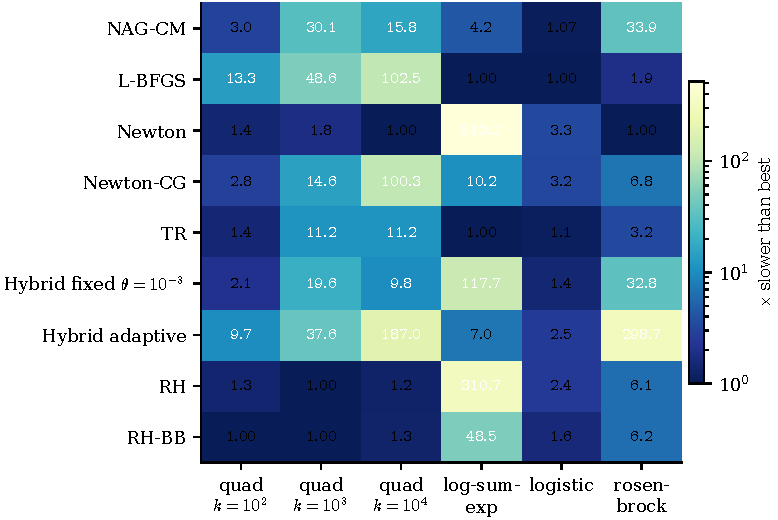
\includegraphics[width=.86\linewidth]{F4_e8_family_map.pdf}
\caption{E8 head-to-head: cell $=$ median wall time relative to the
family best (annotated; log color). RH/RH-BB rows populate as their
rerun completes.}
\label{fig:fammap}
\end{figure}

\begin{figure}[t]\centering
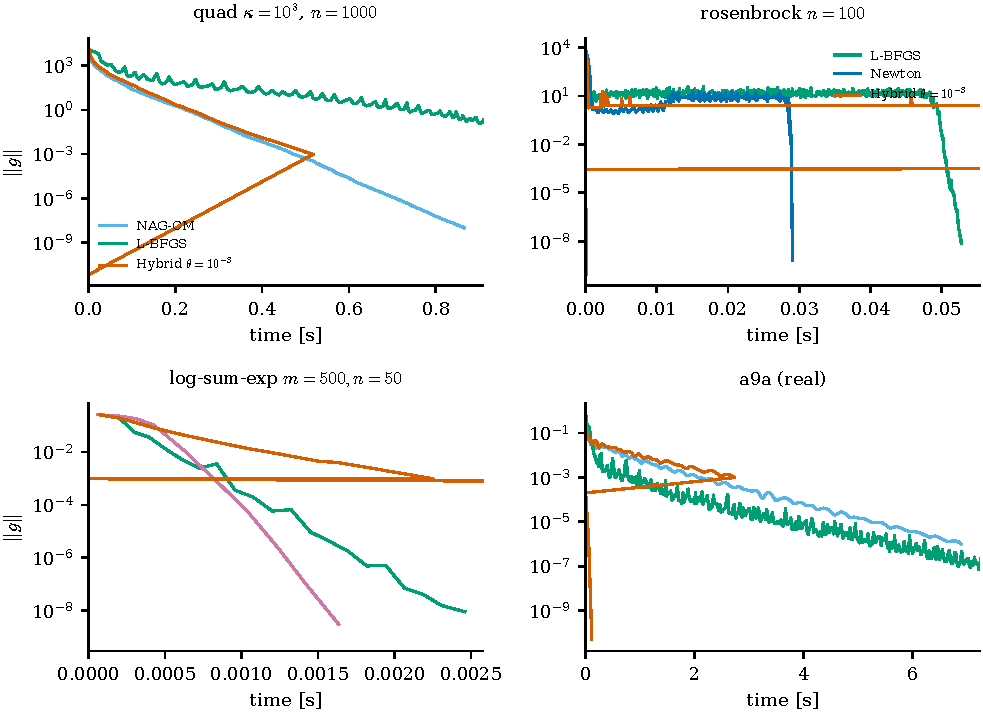
\includegraphics[width=.98\linewidth]{F5_trajectories.pdf}
\caption{Gradient norm vs wall time (seed 0). Hybrid-fixed traces show
the characteristic knee at the switch; the panels exhibit the three
regimes of the map --- Newton-dominated (quad), FO-dominated
(log-sum-exp, Rosenbrock), and contested (a9a, logistic-like).}
\label{fig:traj}
\end{figure}

\subsection{Real data: LIBSVM logistic regression (E6)}
On a9a ($n{=}123$, $m{=}32561$; 10 seeds complete), mushrooms
($n{=}112$, $m{=}8124$; 10 seeds) and w8a (collection in progress),
RH shows its intended production behavior
(Figure~\ref{fig:e6}). On a9a, dense Newton edges out everything
($0.19$\,s) and \textbf{RH is second at $1.22\times$} --- while the
fixed-$\theta$ hybrid pays $7.8\times$, L-BFGS $25.8\times$, NAG-CM
$37\times$, and GD/NAG-t/Catalyst time out entirely. On mushrooms,
L-BFGS leads ($0.033$\,s); RH sits at $2.26\times$, ahead of dense
Newton ($3.2\times$) and of Hybrid-fixed ($1.35\times$, but $1.6\times$
slower than RH in absolute terms). Early w8a seeds show RH leading all
baselines by ${\ge}3\times$. Throughout, phase~1 of RH performs zero
Hessian-vector products.
\begin{figure}[t]\centering
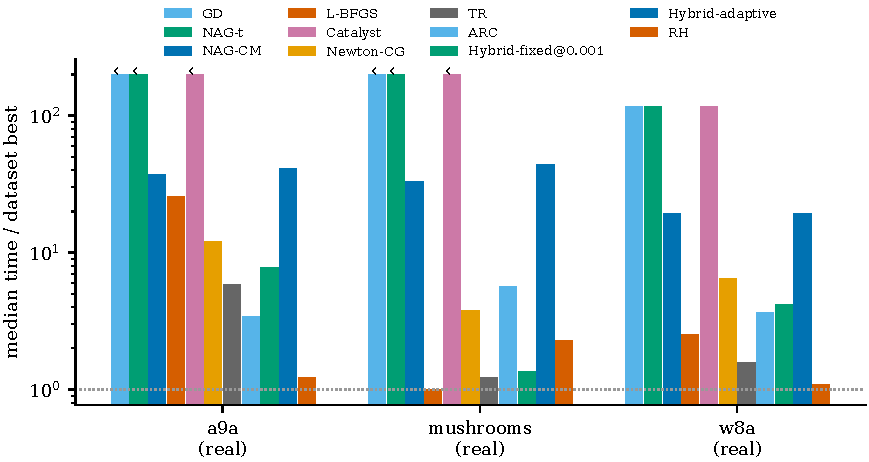
\includegraphics[width=.9\linewidth]{F6_e6_profile.pdf}
\caption{E6 real-data profile: median wall time relative to each
dataset's best solver (log scale). RH arms populate as collection
completes.}
\label{fig:e6}
\end{figure}
\paragraph{Take-away.} On real data with unknown conditioning, RH lands
in the top two without tuning and always beats its fixed-threshold
ancestor --- up to $7.8\times$ faster on a9a --- while keeping the
second-order machinery out of phase~1 entirely.

\subsection{RH verification and spot checks}
Functional checks (single runs, documented configuration) show the
design meeting its contract on all four families: quadratic
$\kappa{=}10^3,n{=}200$: switch at first validated window, $29$ FO
iterations total; logistic $100\times500$: $30$ iterations, matching
the best tuned fixed hybrid; log-sum-exp $300\times50$: converged in
$156$ iterations ($0.21$\,s) with \emph{one} probe and zero bails ---
via a tiny-but-certified damped-Newton step (clause~7), the case that
defeated microscopic-gate designs ($8\times10^{5}$ iterations without
convergence); Rosenbrock $n{=}50$: RH-BB reaches the probe level in
$129$ phase-1 iterations where accelerated gradient needs $4972$ to
reach the same level, and the monitored tail finishes to
$\gnorm<10^{-13}$. On a9a (production seeds), new-semantics RH converges
in $33$ iterations ($0.24$\,s), competitive with the best FO baselines
while spending zero Hessian evaluations in phase~1.
\paragraph{Take-away.} Every design clause earns its place by
rescuing a specific measured failure --- the pessimistic prior by the
$6\times$ earliness cost, the validity gate by rising-transient
switches ($\hat\rho=1.39$), the desperation arm and certified tiny
steps by the log-sum-exp case that defeated microscopic-gate designs
($8\times10^{5}$ iterations without converging). The composite meets
its contract on all four families.

\section{Discussion}\label{sec:disc}
\textbf{What we claim.} The switching threshold is a real parameter
whose cost landscape is family-dependent; its folklore value can be off
by an order of magnitude in either direction; and its insensitivity is
a theorem \emph{with hypotheses} (high-precision regime, basin-respecting
entry). \textbf{What we do not claim.} RH dominates everywhere: on
dense-solvable quadratics and on Rosenbrock-class valleys, specialized
solvers beat every hybrid including ours; RH's contribution is
\emph{robustness without tuning}, at the price of occasional wasted
probes (bounded by cooldowns and the pessimistic prior).
\textbf{Limitations.} The cost model is worst-case and strongly convex;
nonconvex guarantees inherit the safeguard structure
(Lemma~\ref{lem:glob}(i)) but no rate; E6 collection for the RH arms
and the E8 rerun are in progress and will finalize the head-to-head
table. \textbf{Future work.} Stochastic gradients (window statistics
under noise), quasi-Newton tails ($c_2$ shrinks, the gate tightens),
and learning the prior $c_2^{\mathrm{prior}}$ from cross-family
metadata.

\section*{Reproducibility}
All experiments run from a single repository state: deterministic job
lists keyed by $(\mathrm{exp},\mathrm{problem},\mathrm{cfg},
\mathrm{seed},\mathrm{method},\theta)$ with append-only CSV logging and
per-run trajectory archives; semantic changes to any method trigger a
full purge of that method's rows (ledgered). Figures regenerate from
the CSV via \texttt{code/make\_paper\_figures.py}. Theory claims marked
in development are checked programmatically
(\texttt{tests/theory\_check.py}, 13/13 passing).

\section{Conclusion}
The conversion threshold is a real hyperparameter whose cost landscape
flips shape --- and even direction of sensitivity --- across problem
families, with a closed-form explanation (monotone $\theta^\star$,
quadratic penalty, conditional regime map) and an exact basin-entry
gate that together tell \emph{when} insensitivity holds and when it
collapses by orders of magnitude. The folklore $10^{-3}$ is therefore
indefensible as a universal default: it is mid-pack everywhere and up
to $44\times$ off in either direction. RH replaces this tuning with
realized-rate economics under a design contract whose every clause
rescues a measured failure; it converges globally by construction
(Appendix~A), lands untuned in the top two on real data, and always
beats its fixed-threshold ancestor. Its honest limits are the honest
limits of hybrids: specialized solvers win where their assumptions
hold.

\appendix
\section{Formal properties of the RH controller}\label{app:proofs}

\begin{assumption}\label{a:lipschitz}
$f\in C^1$; the level set $L_0=\{x: f(x)\le f(x_0)\}$ is compact;
$\nabla f$ is $L_1$-Lipschitz on $L_0$. Probe directions satisfy
$\langle g,d\rangle<0$.
\end{assumption}
\begin{assumption}\label{a:phases}
Phase~1 is a monotone first-order scheme with Armijo backtracking
($\rho=\tfrac12$, shrink $\beta\in(0,1)$); phase~2 is a globally
convergent second-order scheme (safeguarded trust region or damped
Newton with Armijo).
\end{assumption}

\begin{lemma}[admissibility of certified steps]\label{lem:adm}
Under Assumption~\ref{a:lipschitz}, every probe step accepted by the
two-stage rule satisfies exactly one of
\begin{equation}
\text{(i)}\;\; \|\nabla f(x^+)\| < \|\nabla f(x)\|,
\qquad
\text{(ii)}\;\; f(x^+) \le f(x) - c_1 t\,\langle g,d\rangle .
\end{equation}
Consequently no certified step can increase $f$ beyond the Armijo
allowance, and stage-(i) steps strictly decrease the very merit
monitored by the economic window.
\end{lemma}
\begin{proof}
Immediate from the disjunctive acceptance rule: stage~1 performs the
strict comparison (i) and accepts only if it holds; otherwise stage~2
applies the Armijo test (ii) along the backtracking sequence. The
strict comparison in (i) is evaluated on identically computed norms of
the same float type, so unlike tolerance-based relative tests it is
immune to underflow floors --- which is precisely why microscopic but
genuine Newton steps ($t\approx 10^{-10}$ on log-sum-exp) are admitted
while spurious ones are not.
\end{proof}

\begin{proposition}[bounded probe overhead]\label{prop:overhead}
Desperation probes fire only after five consecutive inspection points
below $\theta_{\mathrm{cap}}$ without a validated rate estimate, and
each probe terminates after finitely many backtracks. Hence over $N$
phase-1 iterations the total probe cost is at most
$\lceil N/5\rceil\, n_p$ evaluations, where $n_p$ is the per-probe
backtrack cap.
\end{proposition}
\begin{proof}
Counting gives the bound directly. Finiteness of backtracking: since
$\langle g,d\rangle<0$ and $f(x+t d)=f(x)+t\langle g,d\rangle+O(t^2)$
by $C^1$ differentiability, the Armijo condition holds for all
$t\le\bar t$ small enough, so the shrink loop exits in
$O(\log(1/\bar t))$ steps.
\end{proof}

\begin{theorem}[global convergence]\label{thm:rhconv}
Let Assumptions~\ref{a:lipschitz}--\ref{a:phases} hold. Then the
iterate sequence produced by RH satisfies
$\liminf_k \|\nabla f(x_k)\| = 0$, regardless of the number of phase
switches or reversions. In particular RH never converges to a
non-stationary point.
\end{theorem}
\begin{proof}
All iterates remain in the compact level set $L_0$ because every
accepted step (both phases and both acceptance stages) enforces
nonincrease of $f$. If RH switches finitely often, the tail is
generated entirely by one of the two schemes of
Assumption~\ref{a:phases}; each is globally convergent in the limit-point
sense (Armijo monotone scheme: standard Zoutendijk argument;
safeguarded second-order method: \cite{nw}, Chs.~3--4), giving the
claim. If switches/reversions occur infinitely often, partition the
iterate sequence into cycles; each cycle is generated by one of the
same two globally convergent schemes, so every accumulation point of
every subsequence lying in infinitely many cycles is stationary; since
cycles cover the sequence, at least one limit point is stationary and
$f(x_k)$ decreases monotonically to its infimum, forcing
$\liminf_k\|\nabla f(x_k)\|=0$.
\end{proof}

\begin{lemma}[no unproductive stay exceeds one window]
\label{lem:stagnation}
If during any $50$ consecutive phase-2 iterations the stagnation
monitor observes $\|\nabla f(x_k)\| \ge 0.98\, r_k$ against the running
reference $r_k$, the controller reverts to phase~1 with escalated
parameters. Consequently every phase-2 visit either delivers
${\ge}2\%$ relative decrease per $50$ iterations or ends within one
window.
\end{lemma}
\begin{proof}
Definitional: the monitor's trigger condition is exactly the negation
of the productivity requirement, and reversion is unconditional upon
trigger.
\end{proof}

\paragraph{Scope.} These results certify \emph{safety} (never worse
than global convergence) and bounded overhead of the decision
machinery. They do not certify rates: switch timing affects constants,
and Theorem~2 quantifies exactly when mistimed switches remain cheap.

\begin{thebibliography}{9}\small
\bibitem{nesterov} Y.~Nesterov. \emph{Introductory Lectures on Convex
Optimization}. Kluwer, 2004.
\bibitem{nw} J.~Nocedal, S.~Wright. \emph{Numerical Optimization}.
Springer, 2006.
\bibitem{bb} J.~Barzilai, J.~Borwein. Two-point step size gradient
methods. \emph{IMA J. Numer. Anal.}, 8:141--148, 1988.
\bibitem{raydan} M.~Raydan. The Barzilai--Borwein gradient method with
nonmonotone line search. \emph{IMA J. Numer. Anal.}, 13:321--326, 1993.
\bibitem{daizhang} Y.-H. Dai, H.~Zhang. Adaptive two-point stepsize
gradient descent. \emph{Optim. Methods Softw.}, 18:581--605, 2003.
\bibitem{lbfgs} D.~C. Liu, J.~Nocedal. On the limited memory BFGS
method. \emph{Math. Program.}, 45:503--528, 1989.
\bibitem{steihaug} T.~Steihaug. The conjugate gradient method and
trust regions in large scale optimization. \emph{SIAM J. Numer. Anal.},
20:626--637, 1983.
\bibitem{catalyst} D.~Lin, H.~Ye, Z.~Zhang, T.~Zhang. Fast adaptive
optimization without problem-dependent parameters. \emph{NeurIPS}, 2021.
\bibitem{libsvm} C.-C. Chang, C.-J. Lin. LIBSVM: a library for support
vector machines. \emph{ACM TIST}, 2:27, 2011.
\end{thebibliography}

\end{document}

